% !TEX root=./whitepaper.tex
\section{Service Marketplace over \projabbrev Compute Network}

As a decentralized AI operating system, \projabbrev also provides a separate platform managing the decentralized computing resources as services.
It organizes the computation resources in a compute network and allows services deployed and registered with verifiability so that users can choose trusted services in the decentralized environment.

\projabbrev compute network is designed as a free marketplace where users and service providers decide the prices of the services through a peer-to-peer fashion. 
The service provider is free to quote their services, and then users are free to choose the services that are priced appropriately for them to use. 
The system assumes that any service result can be verified by the user who submits the request. 
In the trust model, it treats the service providers as more trustworthy than users and less powerful to apply sybil attack. 
Therefore, a user may face the risk of losing the cost of a single request. 
In other words, when a user submits a request and sends fee to smart contract, she may spend the fee but fail to get the service result if the service provider is malicious. 
In this case, the user can choose other service providers in the network to retry the request. 

The service provider should first register into the smart contract with information about the service types that it provides, the price of each type, and the specific verification mechanism. 
When a user wants to access the service, she pre-charges some amount of fee to the smart contract for this service provider. 
The user then can issue requests to the service provider and the service provider decides to respond with the serving results based on whether the remaining fee is enough. 
Any request and response have the signatures of the user and the service provider, respectively. 
The user can verify each response and decide to stop sending further request if the verification is failed. 
The service provider can decide at any point to send the request traces with user’s signature to the smart contract for settlement. 
Once settlement is done, the corresponding portion of the pre-charged fee can be sent to service provider’s account. 

The performance trade-off is how often the service provider submits the settlement request to the smart contract. 
For the high-latency services, the provider can submit settlement per user request. 
But for the low-latency services, the provider may need to batch more user requests for one settlement. 
Another consideration is how the user request trace should be organized as the smart contract input for settlement. 
Plainly submitting all the requests in the trace may involve too much on-chain gas consumption. 
\projabbrev therefore employs zero-knowledge proof mechanism to optimize the on-chain settlement cost. 

\begin{figure}[H]	
	%\vspace{-6mm}
	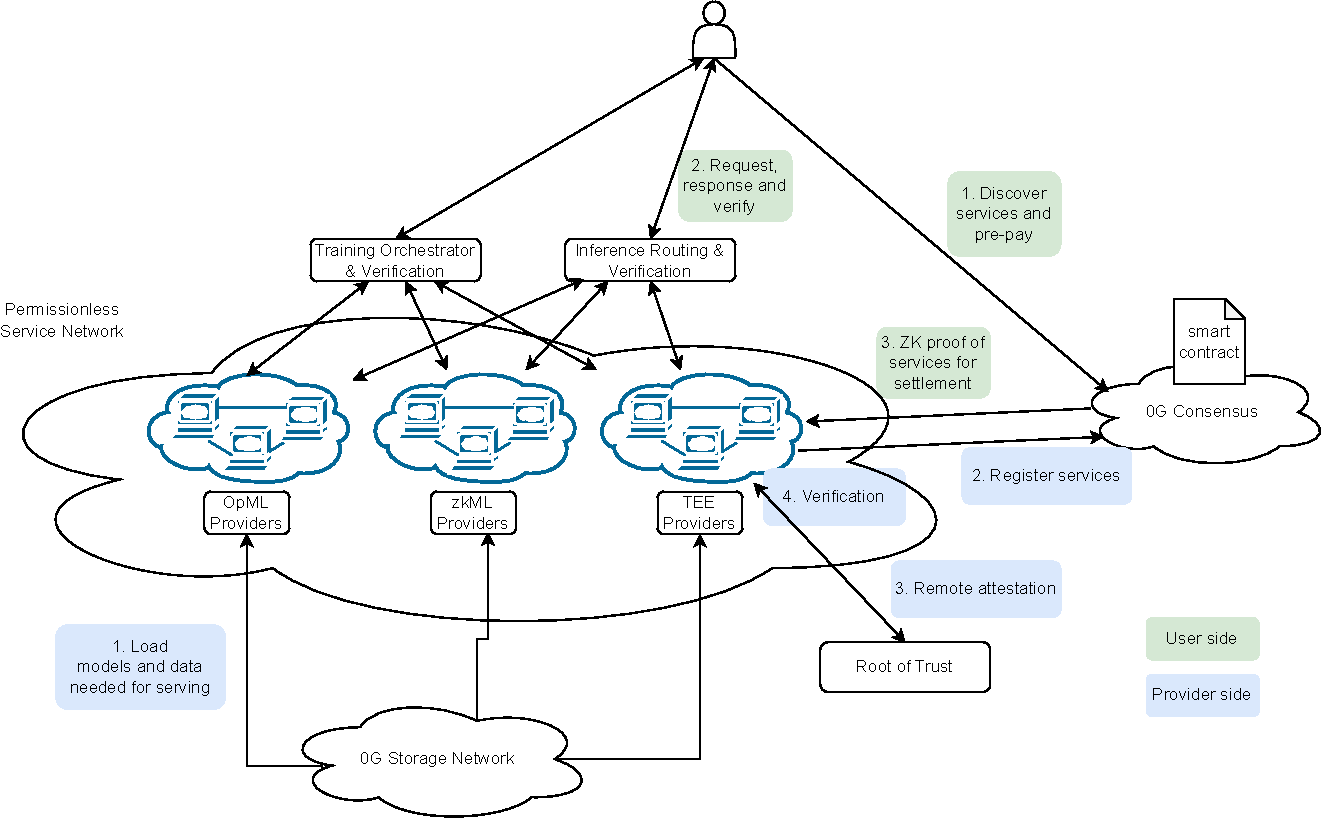
\includegraphics[width=\textwidth]{figure/dAIOS.pdf}
	\caption{The Architecture of \projabbrev Compute Network and Service Marketplace.}
	\label{fig:daios}
	%\vspace{-10mm}
\end{figure}

\projabbrev compute network provides a bunch of useful SDK and APIs for the service providers to easily register their services into the marketplace smart contract, and allows users to conveniently discover appropriate services and interact with them smoothly. 
The services may include AI model inference and training workers, and also the data caching and fetching services.

Together with the \projabbrev storage and DA networks, the \projabbrev compute network and the service marketplace complete the infrastructure foundation of the dAIOS to enable easy migration of AI applications and platforms from Web2 to Web3, and pave the way towards AGI democratization.
